\section{Problem description and data exploration}
\label{sec:problem}

\subsection{Problem description}
The goal of this project is to predict the customer satisfaction level of an unspecified airline, given a set of covariates $X$ that describe several characteristics of the flight, such as service-quality items, type of customer, departure delay and so on, and customer's opinion on the flight, like the rating given to some service quality items. Given the high degree of uncertainty inherent in personal opinions, we chose to adopt a Bayesian logistic regression model\cite{bl_book}. 
%improve this
The Bayesian coefficients are estimated via Markov Chain Monte Carlo (MCMC) methods.

\subsection{Dataset description}
The dataset \cite{kaggle_ds} contains 129{,}881 customer records, described by 22 columns, organised as follows:
\begin{itemize}
    \item \textbf{Target variable}: represents the satisfaction level of customer $i$, denoted $y_i$, which can be either \textit{dissatisfied} or \textit{satisfied} and is encoded respectively as $\{0,1\}$.
    \item \textbf{Categorical variables (3)}: indicate the category of the customer and of the flight to which the record refers. For these variables, one-hot encoding is used.\\ Variable list: \texttt{Customer type, Type of Travel, Class}.
    \item \textbf{Discrete variables (15)}: mostly composed of quality-of-service variables. \\ Variable list (service-quality items excluded): \texttt{Age}.
    \begin{itemize}
        \item \textbf{Service-quality variables (14)}: indicate the various levels of service available throughout the whole journey, from booking to arrival. These variables contain several zeros, which may indicate that the corresponding service was not available during the flight. \\ Variable list: \texttt{Seat comfort, Departure/Arrival time convenience, Food and drink, Gate location, Inflight wifi service, Inflight entertainment, Online support, Ease of Online booking, On-board service, Leg room service, Baggage handling, Check-in service, Cleanliness, Online boarding}.
        \end{itemize}
    \item \textbf{Flight properties (3)}: report the spatial and temporal properties of the flight. They are treated as continuous variables. \\ Variable list: \texttt{Flight distance, Departure delay, Arrival delay}.
    \item \textbf{Modified variables}:
        \begin{itemize}
            \item owing to the extremely high correlation between \texttt{Departure delay} and \texttt{Arrival delay}, we decided to replace the latter with the difference between the two delays, so as to retain the information while reducing the correlation. 
            \item given the high skewness of variables \texttt{Departure Delay} and \texttt{Mid-flight delay}, we decided to correct it trough logarithm transormation. \texttt{Flight Distance} was tested but kept on its original scale as transforming it worsened rather than improving the prediction. 
        \end{itemize}
        Further details on the procedures are given in Appendix \ref{app:data_aug}.
\end{itemize}

\subsection{Dataset exploration}
\label{sec:data_expl}
We begin our exploration by examining the balance of the target variable for the prediction model. As shown in Fig.~\ref{img:sat_balance}, the two classes are fairly balanced, so the use of models more complex than a Bernoulli probability distribution is not justified and will not be pursued.
\begin{figure}[h]
    \centering
    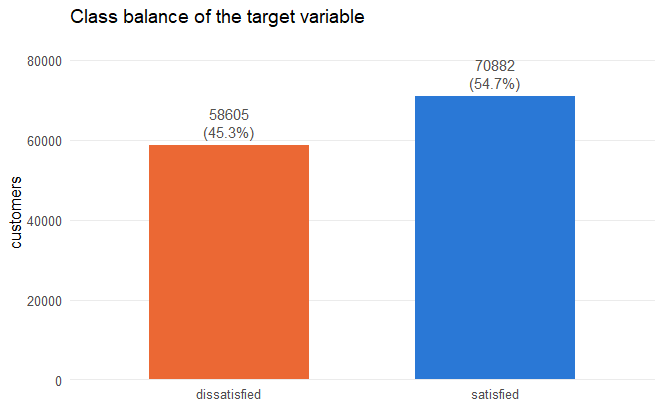
\includegraphics[width=0.4\linewidth]{img/data_expl/sat_balance.png}
    \caption{Target variable class balance}
    \label{img:sat_balance}
\end{figure}

To obtain a first indication of the relationship between the response variable and the remaining covariates, we examine their correlation, as shown in Fig.~\ref{img:full_corr}. Focusing on the service-quality variables (Fig.~\ref{img:qs_corr}), we can distinguish three subgroups of features. The correlation is computed using R's \texttt{corr()} function, which is based on Pearson's correlation coefficient
$$
r_{X,Y} = \frac{\sum (x_i - \bar{x})(y_i - \bar{y})}
               {\sqrt{\sum (x_i - \bar{x})^2 \sum (y_i - \bar{y})^2}}
$$
\begin{figure}
    \centering
    \begin{subfigure}[t]{.48\textwidth}
        \centering
        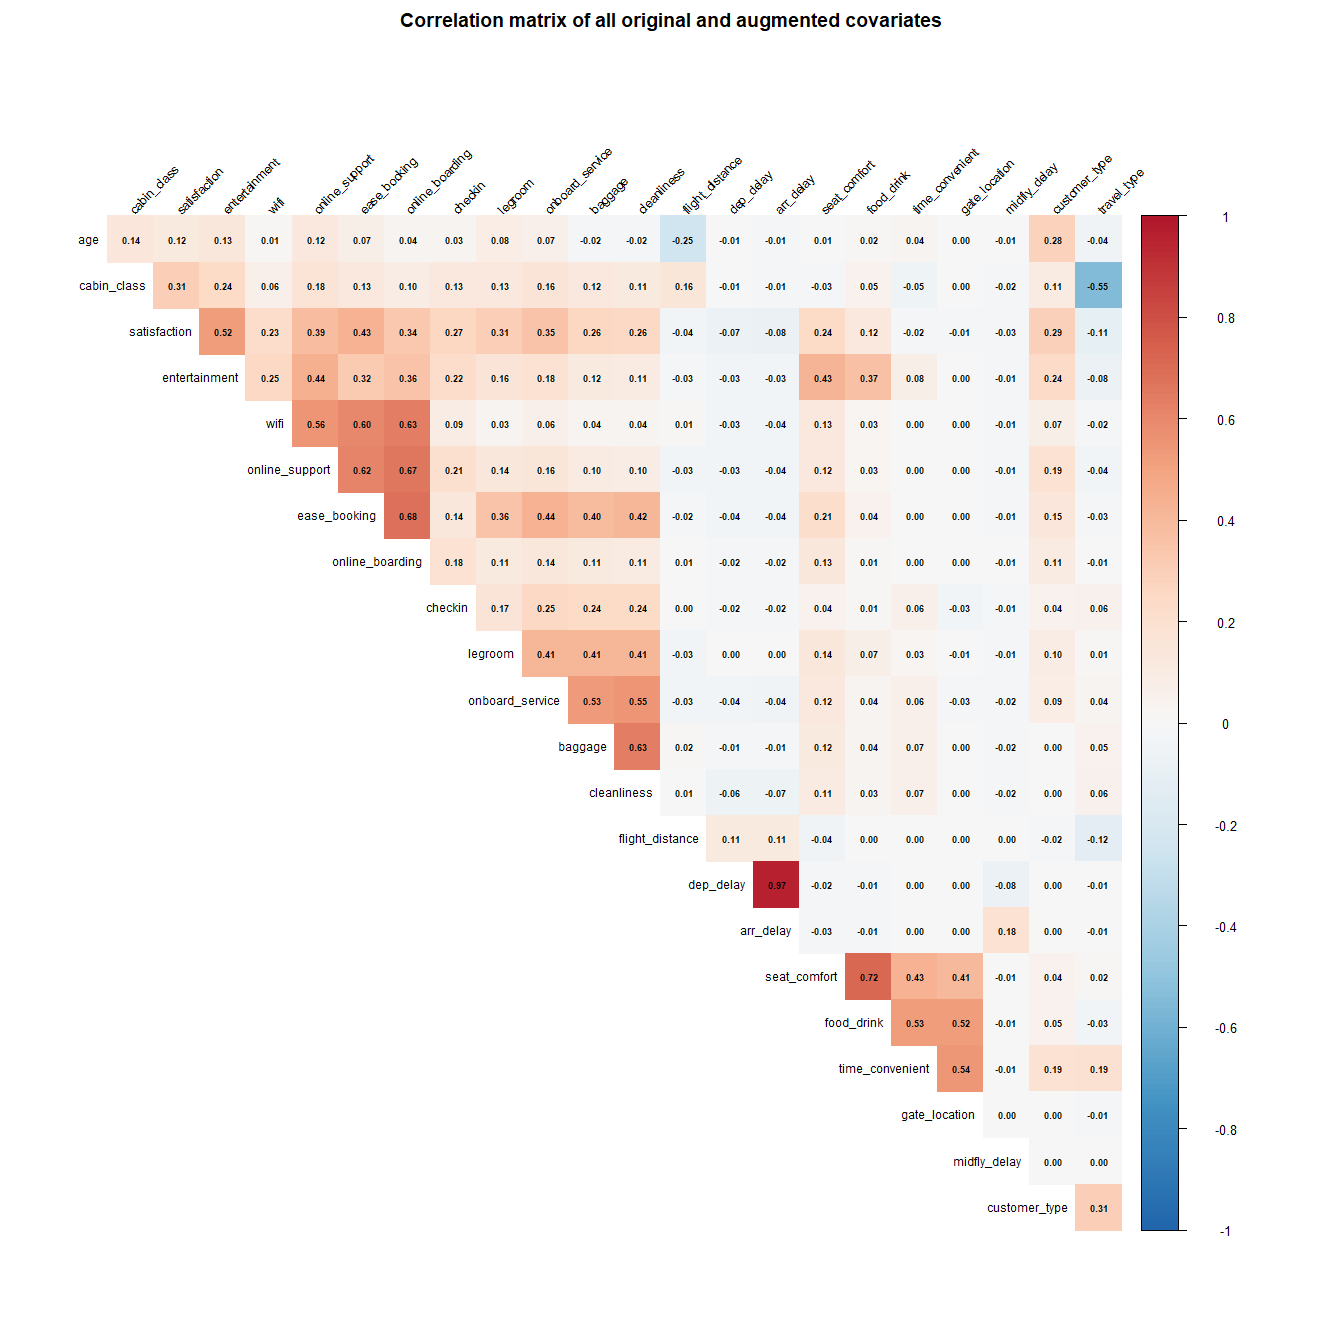
\includegraphics[width=\linewidth]{img/data_expl/full_corr.png}
        \caption{Correlation among all variables, both original and augmented}
        \label{img:full_corr}
    \end{subfigure}
    \hfill
    \begin{subfigure}[t]{.48\textwidth}
        \centering
        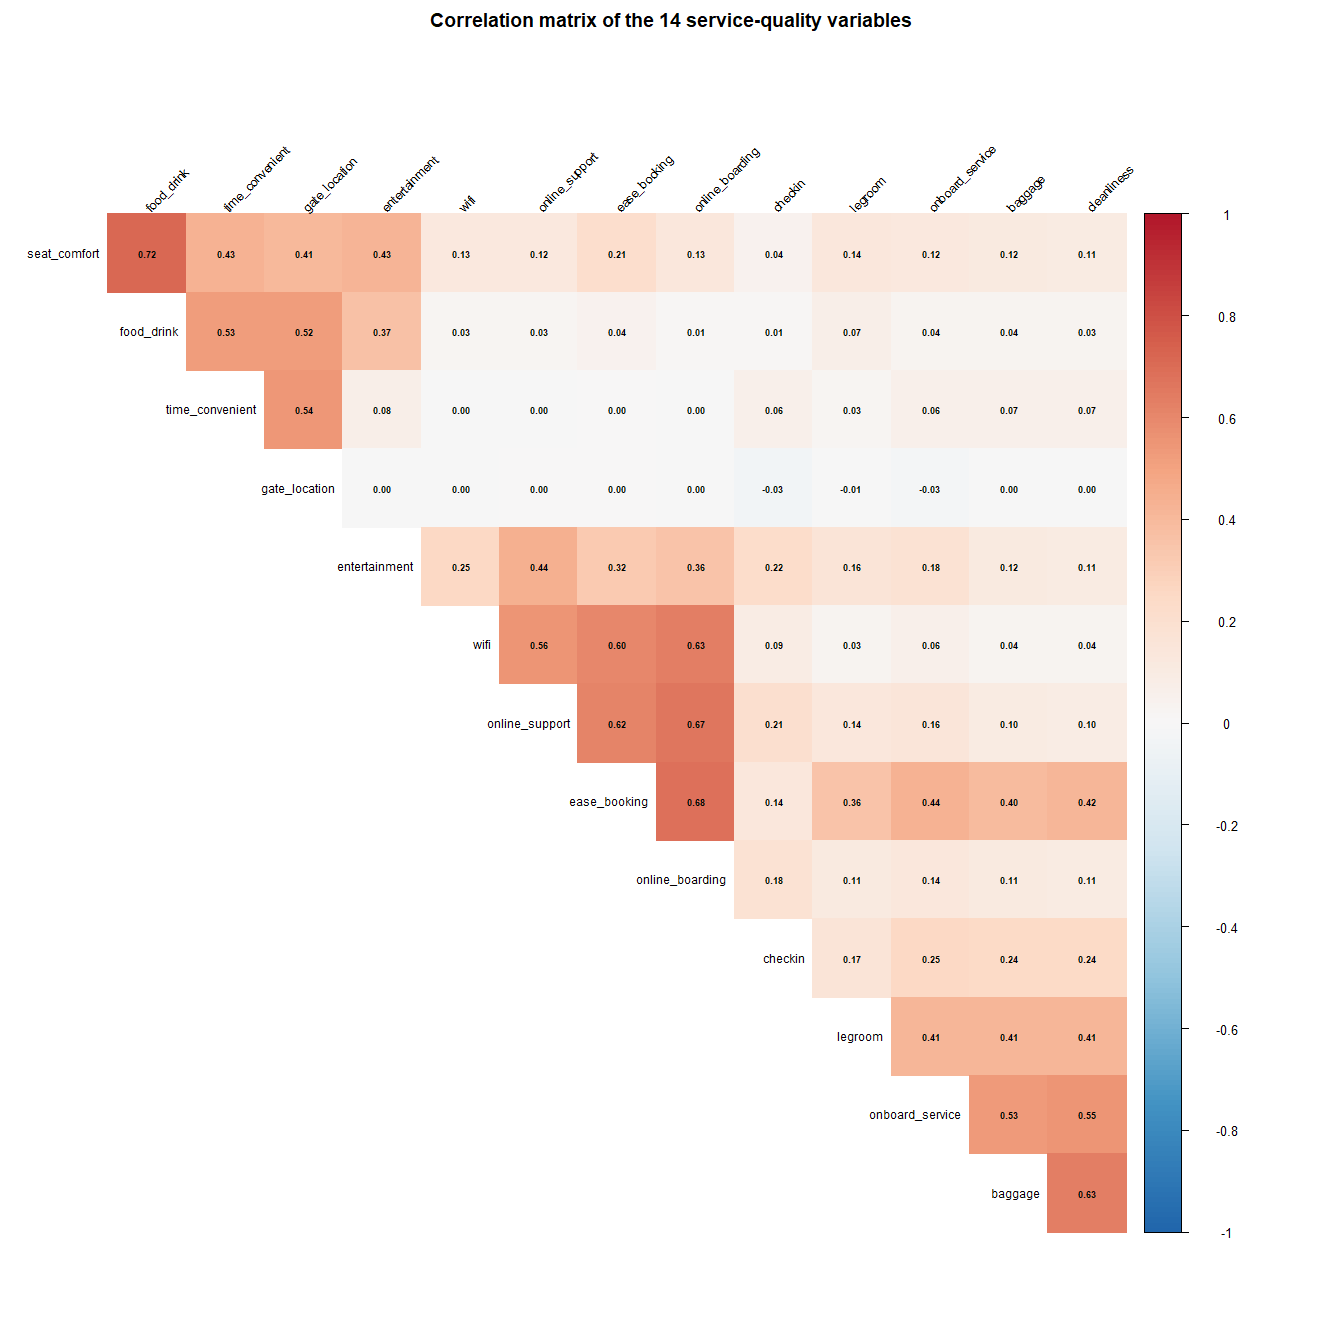
\includegraphics[width=\linewidth]{img/data_expl/qs_corr.png}
        \caption{Correlation among service-quality items}
        \label{img:qs_corr}
    \end{subfigure}
\end{figure}

Tab.~\ref{tab:class_balance} reports the class balance of the remaining categorical variables. Given the imbalance among their levels, we decided to stratify the train--test split of the dataset.
\begin{table}[htbp] 
  \centering
  \caption{Class balance of the categorical covariates}
  \label{tab:class_balance}
  \begin{tabular}{llr}
    \toprule
    Variable & Level & Proportion \\
    \midrule
    Satisfaction  & Dissatisfied      & 0.453 \\
                  & Satisfied         & 0.547 \\
    \addlinespace
    Customer type & Disloyal customer & 0.183 \\
                  & Loyal customer    & 0.817 \\
    \addlinespace
    Travel type   & Business travel   & 0.691 \\
                  & Personal travel   & 0.309 \\
    \addlinespace
    Cabin class   & Eco               & 0.449 \\
                  & Eco Plus          & 0.072 \\
                  & Business          & 0.479 \\
    \bottomrule
  \end{tabular}
\end{table}
